\documentclass[a4paper]{article}

\usepackage[portuguese]{babel}
\usepackage[T1]{fontenc}
\usepackage[utf8]{inputenc}
\usepackage{hyperref}
\usepackage{graphicx}
\usepackage{float}
\usepackage[hypcap]{caption} % makes \ref point to top of figures and tables
\usepackage{amsmath}
\usepackage[nottoc,numbib]{tocbibind}	% adds Biliography to index
%\usepackage[margin=3.3cm]{geometry}

\begin{document}

\pagenumbering{gobble}	% disable page numbering
\begin{titlepage}

	\begin{center}

		
\includegraphics[width=6cm]{./title}\\[3cm]

		\textsc{\LARGE Segurança Informática em Redes e Sistemas}\\[1.5cm]

		\textsc{\Large Projecto}\\[1.5cm]


		{ \huge \bfseries Zero-Day Vulnerability \\[2.5cm] }


		\noindent
		\begin{center} \large
			Gonçalo Ribeiro, 73294\\[5mm]

			António Bacelar de Sousa, 73425\\[5mm]

			Rafael Gonçalves, 73786\\[2.5cm]

		\end{center}

		\begin{minipage}{0.4\textwidth}
			\begin{flushleft} \Large
				Prof. Ricardo Chaves
			\end{flushleft}
		\end{minipage}
		\begin{minipage}{0.4\textwidth}
			\begin{flushright} \Large
				Prof. Miguel Pardal
			\end{flushright}
		\end{minipage}

		\vfill

		{\large \today}

	\end{center}

\end{titlepage}

\tableofcontents
\pagebreak

\pagenumbering{arabic}
\section{Motivação}
Este trabalho tem como motivação fazer um estudo aprofundado de uma zero-day vulnerability, e, desta forma, perceber como funcionam este tipo de ataques e como são tratadas as vulnerabilidades a eles associadas. Para além disso, como motivação também surge o facto de esta ser uma oportunidade para aplicar os conhecimentos adquiridos este semestre na disciplina de Segurança Informática em Redes e Sistemas.

\pagebreak
\section{Objectivos}
\label{sec:objectivos}

\subsection{Antes de 25 de Novembro}

\subsection*{Básico}
Especificar uma vulnerabilidade no Haihaisoft Universal Media Player.
\subsection*{Intermédio}
Realização de um ataque ao software por intermédio da vulnerabilidade especificada.
\subsection*{Avançado}
Investigação e aplicação de métodos que permitam resolver total ou parcialmente a vulnerabilidade do Haihaisoft UMP.

\subsection{Após 25 de Novembro}
Após uma análise cuidada e tentativas de ataque ao Haihaisoft UMP chegámos à conclusão de que era inviável fazer uma \textit{exploit} que fosse consistente entre versões do Windows. Vimo-nos portanto obrigados a escolher outro software com uma vulnerabilidade \textit{zero-day}. De forma a aproveitar o conhecimento adquirido escolhemos um software também vulnerável a \textit{buffer overflows}: o i.FTP. Seguem-se os novos objectivos.

\subsection*{Básico}
Especificar uma vulnerabilidade no software i.FTP.
\subsection*{Intermédio}
Realização de um ou vários ataques ao software tirando proveito da vulnerabilidade especificada.
\subsection*{Avançado}
Tentar eliminar a vulnerabilidade estudada.


\pagebreak
\section{Plano de Trabalho}

\subsection{Semana 1}
Prazo: 07/11/14
\subsubsection{Disponibilidade}
Reduzida devido a avaliações e entregas de projectos de outras UCs.

\subsubsection{Tarefas}
\begin{itemize}
\item escolher um software/website com uma vulnerabilidade activa
\item definir os parâmetros iniciais do projecto
\end{itemize}

\subsubsection{Trabalho Realizado}
Nesta semana procurámos listas de software/websites com vulnerabilidades activas e escolhemos o Haihaisoft Universal Media Player\footnote{\url{http://www.haihaisoft.com/hup.aspx}}, um leitor universal de ficheiros multimédia, como objecto de estudo deste projecto. Este software é desenvolvido para Windows e é software aberto.

Foram também delineados os objectivos deste projecto (Secção~\ref{sec:objectivos}).

\subsection{Semana 2}
Prazo: 14/11/14
\subsubsection{Disponibilidade}
Reduzida devido a avaliações e entregas de projectos de outras UCs.

\subsubsection{Tarefas}
\begin{itemize}
\item preparar uma máquina virtual que possa ser usada ao longo do projecto
\item testar a \textit{proof of concept} (POC) da vulnerabilidade zero-day
\end{itemize}

\subsubsection{Trabalho Realizado}
Tendo-se verificado que o Haihaisoft Universal Player funciona exclusivamente em Windows foi esse o sistema operativo escolhido para instalar na máquina virtual. Como o Windows é software pago teve-se em conta esse factor de forma a fazer uma instalação que não tivesse problemas com licenças. Neste sentido, e visto que o Windows 10 Technical Preview foi lançado recentemente, foi esta a versão do Windows que se escolheu instalar na máquina virtual. De seguida instalou-se o Haihaisoft UMP e verificou-se o seu correcto funcionamento.

Uma das coisas que nos impressionou foi o facto de que o Haihaisoft UMP precisa de privilégios de administrador para ser executado. Como tal, e visto que este software é vulnerável a buffer overflows, o código que conseguirmos injectar vai correr com privilégios de administrador deixando a máquina largamente à nossa mercê.

Por fim testámos a POC encontrada na Exploit Database\footnote{\url{http://www.exploit-db.com/exploits/32514/}}. Esta POC consiste num pequeno script escrito em Python. Como tal, instalámos Python na máquina virtual. Tentámos correr o script mas o Python revelava alguns erros. Após correcção desses erros conseguimos gerar 3 ficheiros de exploit. Experimentámos então abrir esses ficheiros no Haihaisoft. Os resultados dos 3 ficheiros foram semelhantes. Com um deles o programa fechou-se mal era aberto. Com os outros dois ficheiros o programa deixava de responder (aparecia o menu do Windows a dar essa informação), e passado algum tempo o programa era fechado. O shellcode introduzido é um conjunto de instruções que ainda não tivemos oportunidade de verificar o que faz. No entanto verificámos que claramente algo de errado acontece com o programa ao abrir os ficheiros de exploit.

\subsection{Semana 3}
Prazo: 21/11/14
\subsubsection{Disponibilidade}
Muito reduzida devido ao teste de SIRS.

\subsubsection{Tarefas}
\begin{itemize}
	\item Identificar o objectivo do código Assembly injectado através de buffer overflow
\end{itemize}

\subsubsection{Trabalho Realizado}
%Examinámos o código fonte de maneira a descobrir o endereço de retorno, de maneira a alterarmos o código de exploit para conseguirmos correr código nosso

Nesta semana analisámos a POC. São escritos bytes com 4 valores diferentes para o ficheiro de \textit{exploit}. Chegámos à conclusão de que os valores dos bytes se referem aos caracteres ASCII A, B e C e que o outro valor é usado como \textit{padding}.

\subsection{Semana 4}
Prazo: 28/11/14
\subsubsection{Disponibilidade}
Maior disponibilidade.
\subsubsection{Tarefas}
\begin{itemize}
	\item Desenvolvimento do código que se serve da vulnerabilidade encontrada para conseguir acesso com privilégios elevados.
\end{itemize}

\subsubsection{Trabalho Realizado}
A primeira conclusão a que chegámos foi que não é possível fazer um stack based overflow. O Windows usa SEH (structured exception handlers) o que faz com que stack based overflows não sejam possíveis, ou seja, fazer um overwrite directo do EIP (instruction pointer) e fazer um RET.

Outra conclusão foi que o buffer cuja capacidade é excedida não é directamente o buffer que recebe a URL mas sim um buffer que contém a URL transformada, após transformação/eliminação de caracteres que não são permitidos em URLs. Isto significa que os valores de bytes que nos é possível escrever ficam muito mais limitados. Mais concretamente de 256 valores de bytes passamos a poder usar apenas cerca de 90 valores. Por outro lado não nos é possível usar o valor \texttt{0x00} porque é o terminador de strings, e portanto se o usarmos o programa para de copiar bytes assim que encontra um byte com esse valor (parando o nosso overflow antes do que queremos).

O Haihaisoft UMP não foi compilado com protecção da SEH. Ou seja em teoria é possível fazermos overflow das estruturas SEH e enganar o programa de forma a que escreva um novo valor no EIP, valor esse escolhido por nós. Para fazermos isto temos que conseguir que o programa execute uma sequência de instruções POP POP RET que tem que estar em código não compilado com protecção de SEH. Neste caso o próprio executável não tem esta protecção pelo que esta sequência de instruções podia ser uma do próprio programa.

Os programas em Windows têm a memória dividida em 3 componentes. Entre estas, a componente de código é aquela que tem as instruções do programa. Ou seja, é lá que temos que encontrar uma sequência POP POP RET. No entanto, verificámos que os endereços de memória do segmento de código começam todos pelo byte \texttt{0x00}. Isto significa que para enganar o programa de forma a que este salte para a dita sequência de código, teríamos que fazer um overwrite da SEH handler para um endereço cujo primeiro byte é \texttt{0x00}. Ora isso não é possível porque não conseguimos escrever esse valor de byte. Portanto, não conseguimos que seja executada a sequência de instruções necessária para que conseguíssemos alterar o EIP para uma zona de memória controlada por nós de forma a executar uma \textit{exploit}.

Decidimos então alterar o alvo de estudo do nosso projecto do Haihaisoft UMP para outro zero-day.


\subsubsection{Novo Paradigma -- i.FTP}
Consultámos a Exploit Database\footnote{\url{http://www.exploit-db.com}} de forma a encontramos um \textit{zero-day} novo. O candidato que escolhemos foi o i.FTP\footnote{\url{http://www.memecode.com/iftp.php}}. Trata-se de um cliente de FTP que apresenta vulnerabilidades de \textit{buffer overflow} (decidimos manter o tipo de vulnerabilidade a ser explorada).

O referido site oferece uma POC para esta vulnerabilidade. Após análise dessa POC concluímos que a vulnerabilidade resulta do carregamento de um ficheiro de configurações do programa -- Schedule.xml. Existe um campo nesse ficheiro que se refere ao tempo para o qual queremos agendar uma transferência. Esse campo é susceptível a \textit{overflows}.

Fizemos uma análise da vulnerabilidade e conseguimos executar uma \textit{exploit} (abrir a calculadora do Windows). Esta \textit{exploit} não é muito interessante e portanto vamos tentar elaborar outra que o seja.

Quando corremos o programa a calculadora é imediatamente aberta e o programa termina com a janela do Windows que diz que o programa não responde. Gostávamos de evitar que o programa terminasse de forma a que não seja perceptível que algo de errado se passou. A calculadora não é afectada pela terminação do i.FTP, ou seja a \textit{exploit} continua a correr mesmo com o fecho do i.FTP.


\subsection{Semana 5}
Prazo: 05/12/14
\subsubsection{Disponibilidade}
Média.
\subsubsection{Tarefas}
\begin{itemize}
	\item Elaborar um ataque mais interessante;
	\item Evitar que o programa deixe de responder;
	\item Tentar eliminar a vulnerabilidade;
	\item Conclusão do presente documento.
\end{itemize}


\section{SEH Based Overflow -- Passo a Passo}

Nem sempre é possível fazer uma stack based exploit. No entanto no Windows às vezes é possível fazer um ataque com base na SEH (structured exception handling). A SEH é basicamente uma lista ligada de registos relativos às excepções de um programa. Mesmo que um programa não tenha exception handling existe sempre uma handle na SEH que pertence ao Windows e é usada se a excepção não for apanhada por outra handle da SEH.

Cada registo da SEH tem dois ponteiros: um deles aponta para o código a correr no caso da excepção se verificar (SE handler); o outro aponta para a estrutura seguinte da SEH.

A função que é chamada no caso de ocorrer uma excepção tem a particularidade de receber quatro argumentos sendo que um desses argumentos é a ``establisher frame'' cujo valor é o endereço em que se encontra o endereço para a próxima estrutura da SEH. Este endereço é o terceiro elemento no topo da pilha quando a função é chamada. Isto significa que se após a chamada da função for executada uma sequência de instruções POP POP RET o registo EIP passa a apontar para o endereço imediatamente antes da SE handler. Há portanto a possibilidade de conseguirmos executar código visto que com o overflow conseguimos controlar tanto o valor da SE handler como o valor do ponteiro para a próxima estrutura da SEH.

Os passos necessários para fazer uma SEH based exploit são:

\begin{enumerate}
	\item descobrir aproximadamente a partir de que tamanho de input o programa crasha -- exemplo: o programa não apresenta problemas com um input de 1000 caracteres mas sim com um de 2000 
	\item verificar se o programa é vulnerável a ataques via SEH -- se não for não vale a pena continuar
	\item determinar o offset da SEH
	\item encontrar um endereço com uma sequência de instruções POP POP RET
	\item verificar qual a melhor localização da stack para escrever o shellcode
	\item escrever as instruções necessária para fazer um ou vários saltos até à localização do shellcode
	\item escrever o shellcode, sem caracteres terminadores e outros que não seja possível usar
	\item testar a exploit
\end{enumerate}

De seguida descreve-se brevemente como se pode executar cada passo. O debugger usado é o Immunity Debugger. Outro programa auxiliar é o Metasploit.

\paragraph*{Programa vulnerável a SEH?} Usando o plugin \texttt{mona} é possível determinar facilmente quais os módulos não compilados com SafeSEH. Para tal, após instalação do \texttt{mona} basta executar o seguinte comando:

	\texttt{!mona nosafeseh}

No caso do i.FTP vemos que existem dois módulos carregados pelo programa que não têm SafeSEH: \texttt{iftp.exe} e \texttt{Lgi.dll}. Podemos também ver quais os endereços de memória do seu código.

\paragraph*{Determinar offset da SEH} O offset da SEH pode ser determinado com o auxílio do comando \texttt{pattern-create} da ferramenta do Metasploit. Esta ferramenta gera uma sequência de bytes sem repetições, em que se torna fácil descobrir o offset de conjuntos de vários bytes.

	\texttt{ruby pattern\_create.rb 2000}

2000 deve ser substituído pelo número de bytes que se quiser para a sequência. Esse valor deve ser suficientemente grande para o programa crashar.

Usando o debugger para examinar o overflow podemos verificar qual o valor escrito no ``Pointer to the next SEH record'' (nSEH). O offset desse valor desde o início do buffer pode depois ser obtido com:

	\texttt{ruby pattern\_offset.rb Au0A}

em que Au0A é o valor escrito no sítio do ponteiro anteriormente referido para no caso do i.FTP. Ficamos a saber que o offset do início da estrutura é 600.

\paragraph*{Encontrar POP POP RET} Temos que encontrar uma sequência POP POP RET num dos módulos que não tenha SafeSEH. Existem várias formas de o fazer. A mais simples é pesquisar uma sequência de comandos no disassembler fazendo Search for > Sequence of commands (CTRL + S) e escrever nessa janela o que se pode ser na Figura~\ref{find_POPPOPRET}.

\begin{figure}
	\centering
	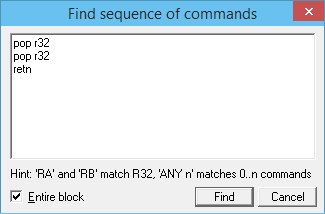
\includegraphics[scale=1]{find_POPPOPRET}
	\caption{procurar uma sequência POP POP RET}
	\label{find_POPPOPRET}
\end{figure}

Uma vez encontrada essa sequência há que anotar o seu endereço para o usar mais tarde. No nosso caso anotámos \texttt{0x1001A24A}, pertencente ao \texttt{Lgi.dll}.

\paragraph*{Melhor localização para o shellcode} A melhor localização para o código do shellcode varia com a sua dimensão e qual o número de bytes na stack que temos sobre o nosso controlo. No caso do i.FTP o offset do último byte sobre o qual temos controlo é cerca de 1360 pelo que devemos ter espaço que chegue para o nosso shellcode a seguir ao registo da SEH. Deferimos então que o shellcode será colocado a seguir ao registo da SEH que está sobre nosso controlo.

\paragraph*{Escrever instrução de salto} Para este passo existem várias opções. É possível fazer compilar uma instrução de salto e usá-la. Mas como neste caso se trata apenas de uma instrução optámos por usar uma referência de x86 para identificar o opcode a usar. Só precisamos de salta para o endereço a seguir à ao registo da SEH. Para isso basta um salto de no máximo 8 bytes visto que esse é o tamanho total do registo da SEH. Consultámos \cite{AMD64vol3_2013} e \cite{refx86asm} e chegámos à conclusão de que para fazer um near JUMP o opcode é \texttt{0xEB} e que o byte seguinte é o valor do salto.

No nSEH escrevemos por exemplo \texttt{0xEB069090} ou \texttt{0x9090EB04} (\texttt{0x90} são NOPs), ou seja podemos salta ou 6 ou 4 bytes dependendo do alinhamento que dermos à instrução near JUMP. A seguir à SEH começamos a escrever o shellcode e é para lá que vamos saltar.

\paragraph*{Escrever o shellcode} Para escrever a exploit podemos usar uma ferramenta do Metasploit, o \texttt{msfpayload}. Este programa gera vários shellcodes para diferentes sistemas operativos.

Um exemplo clássico é o de um shellcode que abre uma calculadora do Windows:

	\texttt{ruby msfpayload windows\/exec CMD=calc.exe R}

No entanto, o shellcode gerado pode conter alguns caracteres que não nos é possível usar (caracteres terminadores de strings) e outros dependendo do caso. Os caracteres terminadores de strings são \texttt{0x00}, \texttt{0x0A} e \texttt{0x0D}. Tem que ser encontrado um shellcode alternativo sem esses caracteres, o que pode ser feito com:

	\texttt{ruby msfpayload windows\/exec CMD=calc.exe R | ruby msfencode \\ -b `\textbackslash x00\textbackslash x0A\textbackslash x0D' -t N}

Verificámos que no caso do i.FTP outro carácter que parece terminar o overflow é o \texttt{0x26}, pelo que esse carácter também foi excluído.

O output resultante está pronto a ser usado como shellcode para o SEH based overflow.


\pagebreak
\section{Resultados}

\subsection{Esperados}
\subsection{Obtidos}


\pagebreak
\bibliographystyle{plain}
\nocite{CorelanTeam, refx86asm, genSEHexploits, AMD64vol3_2013}
\bibliography{CorelanTeam,refx86asm,genSEHexploits,AMD64vol3_2013}	% no spaces between commas!

\end{document}
